% Chapter Template

\chapter{Improving the Output} % Main chapter title

\label{Chapter5} % Change X to a consecutive number; for referencing this chapter elsewhere, use \ref{ChapterX}

%----------------------------------------------------------------------------------------
%	SECTION 1
%----------------------------------------------------------------------------------------
\begin{itemize}
    \item Create simple log
    \item Create tool to render graphics
    \item Example images
\end{itemize}

\begin{itemize}
    \item \emph{How to get render the output: what to do?}
    \item First, create a simple log
    \item Get the layout
    \item Create dot file of layout
    \item Sort by major and minor events
\end{itemize}

\textbf{Add intro. Why we're doing this, etc.}

\section{Creating a Simple Log}
\begin{itemize}
    \item \#Reasoning behind doing this
    \item \#Loop through file
    \item \#Filter each line, return appropriate line type
    \item \#Print in proper format
    \item   Add issues: LBARD T+ etc.
    \item \#Show development of output format
    \item \#Talk about what events, why they were selected
    \item \#Show output log screenshot
    \item Link with the test - run in the 'finally' section
\end{itemize}

The first step in improving the output of the test framework is improving the log output.
To do this, it was decided that a simple log file should be created for several reasons.
The log files produced by the test framework have a considerable amount of detail contained within them, however this comes at the cost of being incredibly large - even a relatively simple test such as DualType (produced in the previous section) can create log files of 4,000+ lines.
More than that, the log files produced are very difficult to follow, as they are ordered by log file, then chronologically.
Meaning that following a chain of events between multiple nodes becomes a process of consistently switching between sections of log file.
\todo{Add more; formatting, timestamp, etc.}

To fix this, the simple log will require six main features.
\begin{itemize}
    \item Consistent formatting
    \item Chronological ordering by timestamp
    \item Reduce amount of information to only useful info
    \item Machine \emph{and} human readable layout information
    \item Log traceability to original log file
    \item Support all pre-existing topology tests
\end{itemize}


Several options exist for creating a simple log.
The first is to modify the pre-existing codebase of LBARD, Servald, Fakeradio, and the test framework, and modify their logging to meet the above requirements.
This is not considered to be a useful use of this thesis, as this would require changing large parts of the codebase for these programs for a relatively mild improvement, as well as modifying the code of pre-tested and running devices.

The next is to modify the test framework to process and modify the log lines while the tests are run before piping them to the log file.
While this does solve the issue of the previous proposed solution this would add a large amount of bloat to the test framework that is not required in the vast majority of the tests, and may actually prove to be either impossible or vastly difficult using the Shell scripts of the test framework.
Further, this will increase the run-time for tests unnecessarily.

The final option is to write a program that after a test is run and the log file produced, processes the log file and filters and simplifies it, and outputs a separate, simpler log file. 
This is the method that was undertaken in this thesis. 
The program will be written in C as it needs to be fast, portable, and use minimal external dependencies, as well as it is the language that the majority of the Serval codebase is written in - allowing for future developers to easily maintain and improve the code.

As shown in \figurename{ \ref{fig:chapter5SimpleFlowchart}} the program follows a simple structure.
The specified log file is opened, and the first line is read into memory.
This line is then filtered depending on its content; if the line should be in the simple log, and what type of line it is. \todo{Fix this sentence}
The filtered line is then modified to be in a consistent format, and then the formatted line is written to the output simple log file.
The program repeats these steps with each line in the file until it reaches the end of the file.

\begin{figure}
    \begin{centering}
        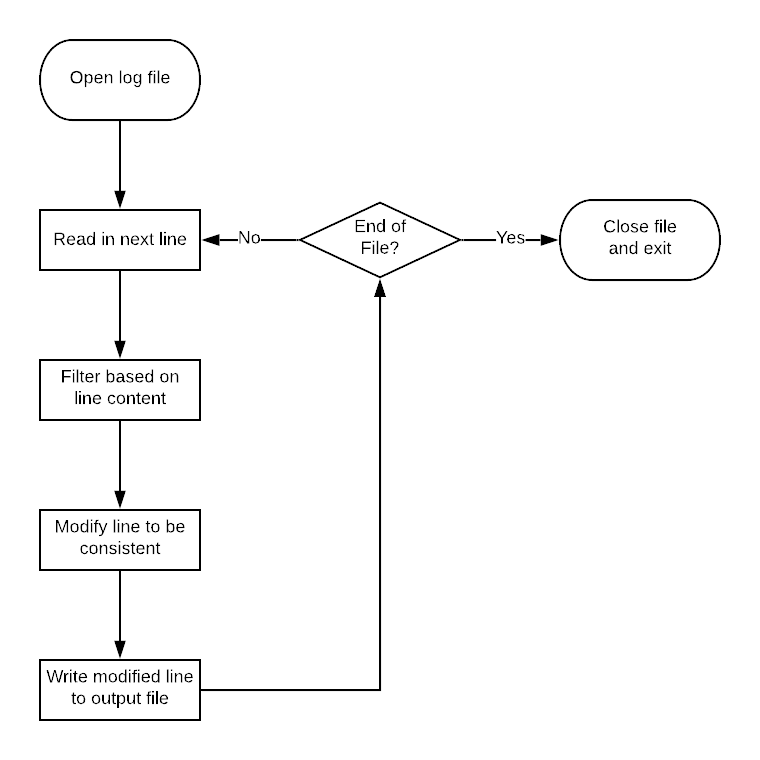
\includegraphics[width=10cm,height=20cm,keepaspectratio]{Figures/Chapter5-SimpleLogFlowchart.png}
        \caption{Flowchart of creating the simple log}
        \label{fig:chapter5SimpleFlowchart}
    \end{centering}
\end{figure}

\subsection{Filtering Lines}
\begin{itemize}
    \item \#What lines we're selecting
    \item Why they are chosen
\end{itemize}

To ensure that the simple log contains only important lines, the input file needs to be filtered.
Filtering the log file allows for the simple log to contain only lines that are crucial to understanding the operating of the test without overwhelming the person examining the log file.

To determine the minimal information required to understand the tests, the output log files of the tests were analysed.
While analysing the output log files, the following list of important events was created.
\begin{itemize}
    \item \textbf{Setup} Start of a process, lbard/fakeradio
    \item \textbf{Setup} Test details
    \item \textbf{Setup} Layout information (WiFi and Fakeradio)
    \item \textbf{Setup} SID information
    \item \textbf{Servald} Sending and receiving packets
    \item \textbf{Servald} Adding manifest
    \item \textbf{LBARD} Neighbour has a bundle
    \item \textbf{LBARD} Send and receive bundles
    \item \textbf{Fakeradio} Any transfer between two nodes
\end{itemize}
\todo{Add why these were chosen?}
This list covers all major aspects of a topology test; transfer of bundles, setup and layout information, sending and receiving general packets (including the tree-sync packets), and some internal logic and processing when packets are sent and received.
With only these important events, it should be possible to locate and isolate issues related to transferring bundles and packets. 
From there, these filtered events should allow a tester to more easily utilise the vastly more expansive and detailed log file. 


Once the desired events had been determined, these then needed to be filtered within the program.
To achieve this, each line in the file is analysed to determine if it is important by examining what substrings the line contains.
A line is accepted if it matches specified criteria; for instance, a line within the Fakeradio process that contains the substring "neighbour has a bundle" would be considered important.

These lines are then sent to the relevant function to be formatted appropriately.

\subsection{Output format}
\begin{itemize}
    \item \#Original log file format
    \item \#How we get consistent format
    \item \#What the output format is
    \item \#Setup section up top
    \item Getting consistent timestamp (talk about issue with LBARD (. instead of :) T+, etc.)
    \item \#Show a screenshot
\end{itemize}

\subsubsection{Formatting lines}
The log files produced by the test framework follow a consistent structure.
The structure always follows the structure of:
\begin{itemize}
    \item the test details, 
    \item the output of the test framework, 
    \item output of Fakeradio, 
    \item output of \emph{each} LBARD process, and finally,
    \item the output of \emph{each} Servald process.
\end{itemize} 

This structure means that filtering each line becomes far simpler, since we only need to track which process (Fakeradio, LBARD, Servald) we are in, and then filter lines within that process that are relevant.
However the test framework log files have one major issue: the format of lines is not consistent between processes.
For instance, the typical Servald line may look like
\begin{center}
    \begin{lstlisting}[breaklines]
DEBUG:[511710] 18:15:34.372 overlay_mdp.c:859:_overlay_send_frame()  {mdprequests} Send frame 68 bytes    
    \end{lstlisting}
\end{center}
while a similar line in LBARD may look like 

\begin{center}
    \begin{lstlisting}[breaklines]
T+25138ms : Sending length of bundle 6A1A3379501553D1* (bundle #0, version 1596098704035, cached_version 1596098704035)
    \end{lstlisting}
        \todo{Make this font smaller?}
\end{center}


As can be clearly seen, there is a huge difference in format between these two lines, and as such these need to be formatted differently.
To achieve this, when a line is filtered as outlined in the previous section, the program returns an integer value representing the type of line that is to be formatted.
With this information, the appropriate function can be called for the line type, so that it can be formatted correctly.

For Servald lines this becomes trivial, simply use the \verb|sscanf| function to extract the important information from the line, format and write this to a variable using the \verb|sprintf| function, and then write this line to the output file. 
However, in the case of LBARD and Fakeradio lines, multiple issues arise due to the formatting of the log files.
The first of these issues is that several lines in LBARD are not timestamped with the time that they occurred, rather they are timestamped with the number of milliseconds since the program started.
This is an issue since this means that the log files can not be easily sorted by timestamp, and also will not be formatted with a consistent format with the other lines.
To fix this, the time that an LBARD instance is started is logged as this is in a normal timestamp format, and when an event with a 'T+' timestamp occurs, the number of milliseconds is added to the original timestamp to produce a timestamp. 
\todo{Fix these sentences}

The other issue with this method is that Fakeradio log lines often are spread over multiple lines.
This means that simply scanning and processing a single line will not produce all the necessary information.
However, when 
\todo{Finish this}

\todo{Add sorting the output}
\subsubsection{Output log file}

Once the log file is produced it follows a consistent format.
The simple log files format begins with the setup section.
The setup section lists all of the essential information for drawing a diagram of the network topology. 
It lists the test details, SIDs of each of the nodes, and all of the WiFi connections and Fakeradio rules. 
An example of the setup section can be seen in \figurename{ \ref{fig:chapter5SimpleLogSetup}}.

\begin{figure}
    \begin{centering}
        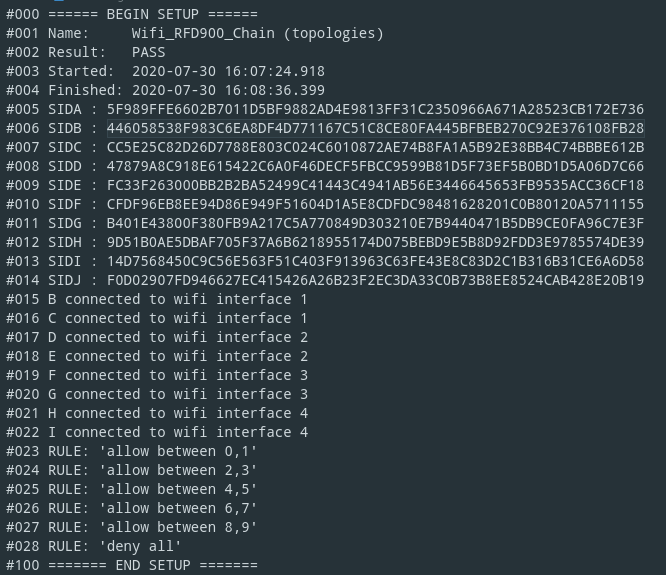
\includegraphics[width=15cm,height=20cm,keepaspectratio]{Figures/Chapter5-SimpleLogSetup.png}
        \caption{Setup section of the simple log}
        \label{fig:chapter5SimpleLogSetup}
    \end{centering}
\end{figure}
After the setup section each line in the log file is ordered by chronological order. 
The lines follow a simple and consistent structure.
\begin{center}
    \begin{lstlisting}[breaklines]
[Timestamp] [Process]:[Instance Letter] [Description]
    \end{lstlisting}
\end{center}
\todo{Maybe have these figures in a lstlisting themselves. Might make the text easier to read?}
This structure can be seen in \figurename{ \ref{fig:chapter5SimpleLogFormat}}
\begin{figure}
    \begin{centering}
        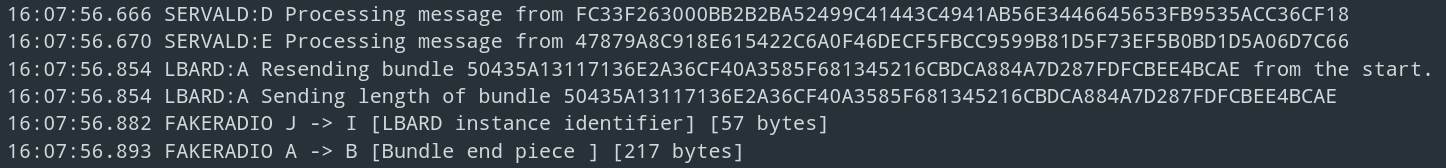
\includegraphics[width=15cm,height=20cm,keepaspectratio]{Figures/Chapter5-SimpleLogFormat.png}
        \caption{Format of simple log events}
        \label{fig:chapter5SimpleLogFormat}
    \end{centering}
\end{figure}


\subsection{Combining with test framework}
\begin{itemize}
    \item Automatically run - in finally section
    \item Need to specify command line arguments - input, output, etc.
    \item Output to log directory
\end{itemize}

\section{Generating a network diagram}
As an improvement to the outputs of the test framework, rendering a network diagram is highly useful, as it allows for testers to better understand the topology that they are testing.
In the test definitions, it is often difficult to understand what the network topology of a given test is.
This is due to the fact that the topology definitions - while easy to understand for a computer - are not particularly friendly for humans to understand, due to their relatively complicated definition.
The topology definition are split into two section, WiFi and Fakeradio, and lists connections only between two nodes - not the entire network.
\todo{Add more / fix this}
To render these diagrams, the layout will need to be extracted from the test definition, then a diagram drawn of this topology.
From this layout, the image will then need to be created and rendered.
There are two main solutions for creating the image: do it using a graphics library, or creating a DOT file and rendering it with Graphviz.
Using a graphics library would provide a high level of control over the creation of the image as graphical elements would need to be defined explicitly and as such are unlikely to have unforseen side-efects as could be expected with using a higher-level solution such as Graphviz.
That said, this would be considerably more complicated and harder to maintain than simply writing DOT files, then using the high-level tools provided by Graphviz to render this DOT file.
DOT files are text files that follow a specified syntax, and are used by Graphviz to render and create graphs.
These files are simple, and both human and machine readable. 
After weighing these options it was decided that despite the far higher level of control possible by using a low-level graphics library, the simplicity and maintainability of creating and rendering DOT files far outweighs this advantage.

\begin{itemize}
    \item Get layout
    \item Decide on DOT file format
    \item Get all combinations of links
    \item Add to dot file
    \item Render 
    \item Why we're hiding fakeradio/WiFI
    \item   (cos we want to animate, doesn't work otherwise)
    \item Show an output diagram (oooh fancy! pictures!)
\end{itemize}






\section{Animating the network diagram}

\subsection{Getting Major and Minor events}
\emph{This is just my thoughts as I was working through the issue. This is not going to be in the final thesis}
I am currently attempting to collect up all of the major (file transfer, show on diagram) and minor (important enough to be on diagram but not on topology) events.
Initially it was planned to get this out of the log file as the log file is processed and the simple log created. 
However, during implementation it was realised that as the original log file is not chronologically ordered, minor events will not easily be tied to a major event.
This is because the majority of the major events occur in fakeradio - when a packet moves from one node to the other.
However, fakeradio - in the log file - comes before LBARD or even Servald.
Thus, the major events that occur in fakeradio will not be tied to any minor event in LBARD or Servald.
There are two possible routes that can be taken to solve this. 
The first, is to simply process the simple log file AFTER it is created, and essentially copy/paste large amounts of code with minimal difference to make it work with processing major/minor lines.
The other alternative is to save all major and minor events while processing the simple log.
The major events can be stored in a struct as planned.
Minor events can simply be a specially formatted string - essentially the same as those in the simple log.

After the simple log is created, the program then sorts both the array of major events, AND the array of minor events.
A blank major event must be created before processing to allow for any minor events that occur BEFORE a major event 
With these both chronologically sorted, the program simply adds any minor events that occur BEFORE a major event to the major event, then once one appears that is LATER than the major event, switches to the next major event.
This loops through until each major and minor event has been processed.
If any minor events are left after the last major event it is added to a blank major event (so nothing gets left off).
A maximum of \emph{n} minor events can be assigned to a major event before it switches over to a new blank major event.

A new array of major events is created after sort. This doubles up on memory, but means that blank events can be added without overwriting other major events.

Does not include broadcast messages because they don't contain enough information.

\subsection{Rendering all of the images}
\begin{itemize}
    \item How we render one
    \item Do in a loop for each of them
    \item LaTeX template, etc.
\end{itemize}

\section{Summary}
\textbf{Add link to next section}